\documentclass[12pt,a4paper]{amsart}
% ukazi za delo s slovenscino -- izberi kodiranje, ki ti ustreza
\usepackage[slovene]{babel}
%\usepackage[cp1250]{inputenc}
\usepackage[T1]{fontenc}
\usepackage[utf8]{inputenc}
\usepackage{amsmath,amssymb,amsfonts}
\usepackage{url}
%\usepackage[normalem]{ulem}
\usepackage[dvipsnames,usenames]{color}
\usepackage{graphicx}
\usepackage{enumitem}
\usepackage{tikz}
%\usetikzlibrary{arrows.meta}
%\usetikzlibrary{shapes.geometric}
\usetikzlibrary{positioning}

% ne spreminjaj podatkov, ki vplivajo na obliko strani
\textwidth 15cm
\textheight 24cm
\oddsidemargin.5cm
\evensidemargin.5cm
\topmargin-5mm
\addtolength{\footskip}{10pt}
\pagestyle{plain}
\overfullrule=15pt % oznaci predlogo vrstico


% ukazi za matematicna okolja
\theoremstyle{definition} % tekst napisan pokoncno
\newtheorem{definicija}{Definicija}[section]
\newtheorem{primer}[definicija]{Primer}
\newtheorem{opomba}[definicija]{Opomba}

\renewcommand\endprimer{\hfill$\diamondsuit$}

\theoremstyle{plain} % tekst napisan posevno
\newtheorem{lema}[definicija]{Lema}
\newtheorem{izrek}[definicija]{Izrek}
\newtheorem{trditev}[definicija]{Trditev}
\newtheorem{posledica}[definicija]{Posledica}


% za stevilske mnozice uporabi naslednje simbole
\newcommand{\R}{\mathbb R}
\newcommand{\N}{\mathbb N}
\newcommand{\Z}{\mathbb Z}
\newcommand{\C}{\mathbb C}
\newcommand{\Q}{\mathbb Q}

% ukaz za slovarsko geslo
\newlength{\odstavek}
\setlength{\odstavek}{\parindent}
\newcommand{\geslo}[2]{\noindent\textbf{#1}\hspace*{3mm}\hangindent=\parindent\hangafter=1 #2}

% naslednje ukaze ustrezno popravi
\newcommand{\program}{Matematika} % ime studijskega programa: Matematika/Finan"cna matematika
\newcommand{\imeavtorja}{Ines Meršak} % ime avtorja
\newcommand{\imementorja}{prof.~dr. Sandi Klavžar} % akademski naziv in ime mentorja
\newcommand{\naslovdela}{Problem londonskega stolpa}
\newcommand{\letnica}{2016} %letnica diplome


% commands
\newcommand{\graf}[1][G]{\ensuremath{#1 = (V(#1), E(#1))}}
\newcommand{\vozlisca}[1][G]{\ensuremath{V(#1)}}
\newcommand{\povezave}[1][G]{\ensuremath{E(#1)}}
\newcommand{\bd}{\ensuremath{|\,}}
\newcommand{\ed}{\ensuremath{\,|}}
% operatorji
\DeclareMathOperator {\stopnja} {deg}




\begin{document}

% od tod do povzetka ne spreminjaj nicesar
\thispagestyle{empty}
\noindent{\large
UNIVERZA V LJUBLJANI\\[1mm]
FAKULTETA ZA MATEMATIKO IN FIZIKO\\[5mm]
\program\ -- 1.~stopnja}
\vfill

\begin{center}{\large
\imeavtorja\\[2mm]
{\bf \naslovdela}\\[10mm]
Delo diplomskega seminarja\\[1cm]
Mentor: \imementorja}
\end{center}
\vfill

\noindent{\large
Ljubljana, \letnica}
\pagebreak

\thispagestyle{empty}
\tableofcontents
\pagebreak

\thispagestyle{empty}
\begin{center}
{\bf \naslovdela}\\[3mm]
{\sc Povzetek}
\end{center}
% tekst povzetka v slovenscini
V povzetku na kratko opi"si vsebinske rezultate dela. Sem ne sodi razlaga organizacije dela -- v katerem poglavju/razdelku je kaj, pa"c pa le opis vsebine.
\vfill
\begin{center}
{\bf The Tower of London problem}\\[3mm] % prevod slovenskega naslova dela 
{\sc Abstract}
\end{center}
% tekst povzetka v anglescini
Prevod zgornjega povzetka v angle"s"cino.

\vfill\noindent
{\bf Math. Subj. Class. (2010):} navedi vsaj eno klasifikacijsko oznako -- dostopne so na \url{www.ams.org/mathscinet/msc/msc2010.html}  \\[1mm]  
{\bf Klju"cne besede:} navedi nekaj klju"cnih pojmov, ki nastopajo v delu  \\[1mm]  
{\bf Keywords:} angle"ski prevod klju"cnih besed
\pagebreak


 
% tu se zacne tekst seminarja
\section{Uvod}
Test londonskega stolpa je ena izmed variacij Hanojskih stolpov. Izumil ga je britanski nevropsiholog Tim Shallice leta 1982. Pogosto je uporabljen v psihologiji, saj s pomočjo te igre ugotavljajo stanje pacientove psihe, opazujejo pa lahko tudi napredek bolezni pri npr.\ Parkinsonovih bolnikih. \cite{bib:wikishal}

Osnovna verzija londonskega stolpa vsebuje tri enako velike krogle različnih barv in tri palice. Na prvo palico lahko postavimo samo eno kroglo, na drugo le dve krogli, na tretjo pa tri. Cilj igre je priti iz nekega danega stanja v neko drugo želeno stanje s čim manj koraki. Stanja (in prehode med njimi) lahko opišemo s pomočjo teorije grafov.

Diplomska naloga je razdeljena na tri dele: v prvem delu bom najprej opisala vse pojme, navedla (in nekatere tudi dokazale) vse trditve, izreke in posledice teorije grafov, ki mi bodo v pomoč pri obravnavi problema londonskega stolpa. V drugem delu bom podrobneje opisala klasični londonski stolp in lastnosti pripadajočega grafa, v zadnjem delu pa bom obravnavala posplošeni problem londonskega stolpa.


\section{Osnovni pojmi teorije grafov}

Vsa možna stanja londonskega stolpa in prehode med njimi lahko zelo elegantno opišemo s pomočjo grafov, zato si najprej poglejmo nekaj osnovnih pojmov teorije grafov.

\begin{definicija}
	\emph{Graf} $G$ je urejen par $(\vozlisca, \povezave)$, kjer je $\vozlisca$ končna množica \emph{vozlišč}, $\povezave$ pa množica \emph{povezav} grafa. Povezave so predstavljene kot neurejeni pari vozlišč (neusmerjeni grafi).
\end{definicija}

Obstajajo variacije zgornje definicije, graf je lahko npr.\ usmerjen (povezave so urejeni pari) -- tedaj govorimo o \emph{digrafih}, ima neskončno število vozlišč ali pa več povezav med dvema vozliščema. Dopuščamo lahko tudi zanke: to je povezava oblike $\{v,v\}$, pri čemer je $v$ vozlišče.

Vozlišča grafa predstavimo s točkami v ravnini, povezavo med dvema vozliščema pa kot enostavno krivuljo med ustreznima točkama v ravnini. Preslikavi, ki grafu priredi ustrezne točke in krivulje v ravnini, pravimo \emph{risba grafa} (včasih pa s tem mislimo kar na predstavitev grafa v ravnini). Graf ima lahko več različnih možnih risb -- razlikujejo se lahko npr.\ po tem, katere točke priredimo katerim vozliščem.

\begin{figure}[h]
    \caption{Možna predstavitev grafa v ravnini.}
\end{figure}
    
Če je $e = \{ u,v \}$ povezava, tedaj sta $u$ in $v$ \emph{krajišči} povezave $e$, pišemo tudi $e = uv$; rečemo, da sta $u$ in $v$ \emph{sosednji vozlišči}.

\begin{definicija}
	\emph{Soseščina} vozlišča $u$ je množica vseh sosednjih vozlišč vozlišča $u$:
	\[ N(u) = \{ x\colon ux \in \povezave \} .\]
	\emph{Stopnja vozlišča} $u$ je število vseh vozlišč, ki so mu sosednji: $\stopnja u = |N(u)|$.
\end{definicija}

Če imamo podano stopnjo vseh vozlišč grafa, lahko na enostaven način izračunamo število povezav tega grafa, velja sledeča lema:

\begin{lema}[Lema o rokovanju]
    \label{lema:rokovanje}
    Za vsak graf \graf velja formula
    \begin{equation}
        \sum_{u \in V(G)}\! \stopnja u = 2 \cdot |E(G)|.
        \label{eq:lema-o-rokovanju}
    \end{equation}
\end{lema}

\begin{proof}
    Naredimo si tabelo vozlišč in povezav:
    
    \begin{table}[h]
        \centering
        \begin{tabular}{c|ccc}
            & \ldots & $e_j$ & \ldots \\ \hline
            \vdots & & \vdots & \\
            $v_i$ & \ldots & 1 / 0 & \\
            \vdots & & &
        \end{tabular}
    \end{table}
    
    V prvem stolpcu so našteta vozlišča grafa, v prvi vrstici pa povezave. Na mestu $i,j$ v tabeli zapišemo enico, če je vozlišče $v_i$ eno izmed krajišče povezave $e_j$, in ničlo v nasprotnem primeru. 
    
    Vemo, da ima vsaka povezava dve krajišči, torej sta v vsakem stolpcu natanko dve enici. Če po drugi strani pogledamo število enic v neki vrstici $i$, nam to pove ravno stopnjo vozlišča $v_i$. Ker mora biti rezultat enak, če seštejemo ničle in enice po stolpcih oziroma po vrsticah, sledi formula \eqref{eq:lema-o-rokovanju}.
\end{proof}

\begin{primer}
    \label{primer:sosedi}
    Naj bo graf $G$ podan z \[\vozlisca = \{ 1,2,3,4,5 \}, \quad \povezave = \left\{ \{1,4\},\{1,5\},\{2,5\},\{3,4\},\{3,5\} \right\}.\]
    \begin{figure}[h]
        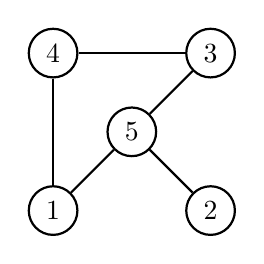
\begin{tikzpicture}
        \begin{scope}[every node/.style={circle,thick,draw}]
        \node (1) at (-1,-1) {$1$};
        \node (2) at (1,-1) {$2$};
        \node (3) at (1,1) {$3$};
        \node (4) at (-1,1) {$4$};
        \node (5) at (0,0) {$5$};
        \end{scope}
        
        \path[-,draw,thick] 
        (1) edge (4)
        (1) edge (5)
        (2) edge (5)
        (3) edge (4)
        (3) edge (5);
        \end{tikzpicture}
        \caption{Graf $G$.}
    \end{figure}
    Soseščina vozlišča 5 je $N(5) = \{1,2,3\}$.
\end{primer}

\begin{definicija}
	Graf $\graf[H]$ je \emph{podgraf} grafa $\graf$, če velja 
	\[ \vozlisca[H] \subseteq \vozlisca \text{ in } \povezave[H] \subseteq \povezave. \]
	Podgraf H grafa G je \emph{inducirani} podgraf, če za vsaki dve vozlišči $x,y\in \vozlisca[H]$ velja: $xy \in \povezave \implies xy \in \povezave[H]$.
\end{definicija}

\begin{primer}
    Če vzamemo graf $G$ iz prejšnjega primera~\ref{primer:sosedi}, potem je graf $H$, ki ima
    
    \[ \vozlisca[H] = \{2,3,4,5\},\quad \povezave[H] = \left\{ \{2,3\},\{2,5\},\{3,4\},\{3,5\} \right\} \]
    
    induciran podgraf grafa $G$.
    
    \begin{figure}[h]
        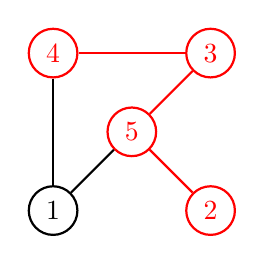
\begin{tikzpicture}
        \begin{scope}[every node/.style={red,circle,thick,draw}]
        \node (1)[black] at (-1,-1) {$1$};
        \node (2) at (1,-1) {$2$};
        \node (3) at (1,1) {$3$};
        \node (4) at (-1,1) {$4$};
        \node (5) at (0,0) {$5$};
        \end{scope}
        
        \path[red,-,draw,thick] 
        (1) edge[black] (4)
        (1) edge[black] (5)
        (2) edge (5)
        (3) edge (4)
        (3) edge (5);
        \end{tikzpicture}
        \caption{Graf $H$ (označen z rdečo barvo) je induciran podgraf grafa $G$.}
    \end{figure}
\end{primer}

Poglejmo si nekaj razredov grafov, ki nam bodo prišli prav v kasnejših definicijah. 

\emph{Pot} na $n$ vozliščih je graf, ki ima dve vozlišči stopnje $1$, medtem ko so preostala vozlišča stopnje $2$.

\emph{Cikel} na $n$ vozliščih (označimo ga s $C_n$) je graf, ki ga dobimo iz poti na $n$ vozliščih tako, da dodamo povezavo med vozliščema stopnje $1$.

\emph{Polni graf} na $n$ vozliščih (označimo ga s $K_n$) je graf, za katerega velja 
\[ uv \in \povezave[K_n] \quad \forall u,v \in \vozlisca[K_n].\] 
Z besedami, vsa vozlišča polnega grafa so med sabo povezana.

\begin{figure}[h]
    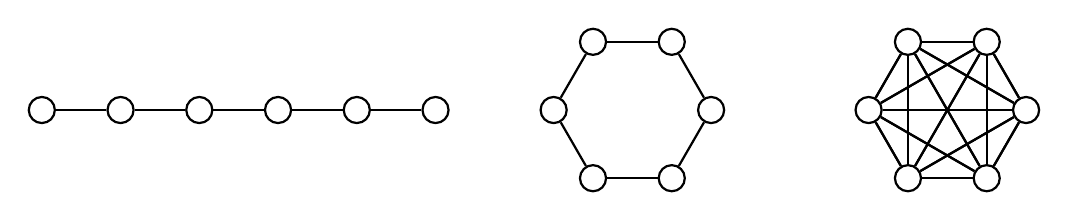
\begin{tikzpicture}
    \pgfmathtruncatemacro{\N}{6}
    \begin{scope}[every node/.style={circle,thick,draw}, every edge/.style={draw,thick}]
        \foreach \x in {1,...,\N}
            \node (\x) at (\x - 4,0) {};

        \foreach \x [remember=\x as \lastx (initially 1)] in {1,...,\N}
            \path (\x) edge (\lastx);
    \end{scope}

    \pgfmathtruncatemacro{\r}{1.1}
    \begin{scope}[xshift=4.5cm, every node/.style={circle,thick,draw}, every edge/.style={draw,thick}]
        \foreach \x in {1,...,\N}
            \node (\x) at (\x*360/\N:\r cm) {};
        \foreach \x [remember=\x as \lastx (initially 1)] in {1,...,\N,1}
            \path (\x) edge (\lastx);
    \end{scope}
    
    \begin{scope}[xshift=8.5cm, every node/.style={circle,thick,draw}, every edge/.style={draw,thick}]
        \foreach \x in {1,...,\N}
            \node (\x) at (\x*360/\N:\r cm) {};
        \foreach \x in {1,...,\N}{%
            \foreach \y in {1,...,\N}{%
                \path (\x) edge (\y);
            }
        }
    \end{scope}
    
%    \begin{scope}[xshift=8.5cm, every node/.style={circle,thick,draw}]
%    \node (1) at (-0.7,1) {};
%    \node (2) at (0.7,1) {};
%    \node (3) at (1.5,0) {};
%    \node (4) at (0.7,-1) {};
%    \node (5) at (-0.7,-1) {};
%    \node (6) at (-1.5,0) {};
%    \path[-,draw,thick]
%    (1) edge (2)
%    (1) edge (3)
%    (1) edge (4)
%    (1) edge (5)
%    (1) edge (6)
%    (2) edge (3)
%    (2) edge (4)
%    (2) edge (5)
%    (2) edge (6)
%    (3) edge (4)
%    (3) edge (5)
%    (3) edge (6)
%    (4) edge (5)
%    (4) edge (6)
%    (5) edge (6);
%    \end{scope}    
    \end{tikzpicture}
    \caption{Primer poti (levo), cikla (sredina) in polnega grafa (desno) na šestih vozliščih.}
\end{figure}

\begin{definicija}
    Graf $G$ je \emph{dvodelen}, če lahko množico njegovih vozlišč razbijemo na dva dela ($V_1,V_2$) tako, da ima vsaka povezava grafa $G$ eno krajišče v $V_1$ in drugo v $V_2$.
\end{definicija}

Pri polnem dvodelnem grafu z $n$ vozlišči v prvi množici, recimo ji $V_1$, in $m$ vozlišči v drugi množici, recimo ji $V_2$, je vsako vozlišče iz množice $V_1$ povezano z vsakim iz $V_2$, medtem ko znotraj množic vozlišča niso povezana. Tak graf označimo s $K_{n,m}$.

\begin{figure}[h]
    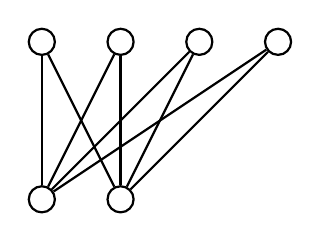
\begin{tikzpicture}
    \pgfmathtruncatemacro{\M}{2}
    \pgfmathtruncatemacro{\N}{4}
    \begin{scope}[every node/.style={circle,thick,draw}, every edge/.style={draw,thick}]
        \foreach \x in {1,...,\N}
            \node (\x) at (\x,1) {};
        \foreach \x [count=\xi from \N+1] in {1,...,\M}
            \node (\xi) at (\x,-1) {};
        
        \foreach \x in {1,...,\N}
            \foreach \y [count=\yi from \N+1] in {1,...,\M}
                \path (\x) edge (\yi);
    \end{scope}
    \end{tikzpicture}
    \caption{Na sliki je polni dvodelni graf $K_{2,4}$.}
\end{figure}

\begin{definicija}
	Naj bosta $\graf$ in $\graf[H]$ grafa. 
	Preslikava $f\colon \vozlisca \to \vozlisca[H]$ je \emph{izomorfizem}, če je bijektivna in velja
	\[ uv \in \povezave \iff f(u)f(v) \in \povezave[H],\quad \forall u, v \in \povezave. \]
	Grafa $G$ in $H$ sta \emph{izomorfna}, če obstaja izomorfizem $G \to H$. Oznaka: $G \cong H$.
\end{definicija}

\emph{Pot v grafu} $G$ je podgraf grafa $G$, ki je izomorfen poti.
\emph{Cikel v grafu} $G$ je podgraf grafa $G$, ki je izomorfen ciklu. 

\subsection{Povezanost grafa}

\emph{Sprehod} v grafu $G$ je zaporedje vozlišč $v_1, v_2, \ldots, v_k$, tako da velja $v_i v_{i+1} \in E(G),$ pri čemer je $1 \leq i \leq k-1$. Če označimo $x = x_1$ in $y = x_k$, potem takemu sprehodu rečemo $x,y$-sprehod.

Sprehod je \emph{enostaven}, če so vsa njegova vozlišča različna. Enostaven sprehod inducira podgraf, ki je izomorfen poti (torej pot v grafu).

\begin{figure}[h]
%    \includegraphics[width=200pt]{img/enostaven-sprehod1.png}
%    \includegraphics[width=200pt]{img/enostaven-sprehod2.png}
    \caption{Enostaven sprehod in pot v grafu, ki jo inducira.}
\end{figure}

Naj bo $G$ graf in $\sim$ relacija, definirana na kartezičnem produktu $\vozlisca \times \vozlisca$:
\[ x \sim y \ \stackrel{\text{def}}{\equiv} \ \exists \ x,y \text{-sprehod.} \]

Preprosto lahko preverimo, da je relacija $\sim$ ekvivalenčna. Sledi, da relacija $\sim$ množico vozlišč grafa G razbije na ekvivalenčne razrede. Podgrafi, inducirani s temi razredi, so \emph{komponente} grafa $G$.

\begin{definicija}
	Graf je \emph{povezan}, če ima le eno komponento. Povedano drugače, za poljuben par vozlišč mora obstajati sprehod med njima.
\end{definicija}

\begin{figure}[h]
    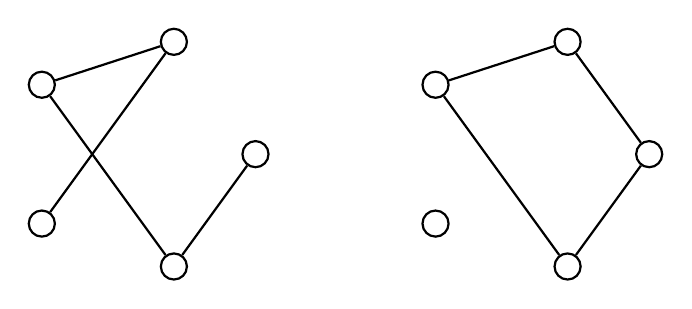
\begin{tikzpicture}
        \begin{scope}[every node/.style={circle,thick,draw}, every edge/.style={draw,thick}]
        \pgfmathtruncatemacro{\N}{5}
            \foreach \x in {1,...,\N}
                \node (\x) at (\x*360/\N:1.5cm) {};
            
            \foreach \x[remember=\x as \lastx (initially 3)] in {1,2,4,5}
                \path (\x) edge (\lastx);
        \end{scope}
        
        \begin{scope}[xshift=5cm,every node/.style={circle,thick,draw}, every edge/.style={draw,thick}]
            \pgfmathtruncatemacro{\N}{5}
            \foreach \x in {1,...,\N}
                \node (\x) at (\x*360/\N:1.5cm) {};
        
            \foreach \x[remember=\x as \lastx (initially 5)] in {1,2,4,5}
                \path (\x) edge (\lastx);
        \end{scope}
    \end{tikzpicture}
    \caption{Povezan (levo) in nepovezan (desno) graf.}
\end{figure}

Če je $G$ povezan graf, lahko definiramo \emph{razdaljo} $d_G(u,v)$ med vozliščema $u$ in $v$ kot najmanjše možno število povezav na neki $u,v$-poti.

Definirajmo še \emph{premer} grafa kot največjo minimalno razdaljo med pari vozlišč. Enostavneje povedano to pomeni: če vzamemo poljubno vozlišče v grafu, potem lahko pridemo do drugega poljubnega vozlišča preko $d$ ali manj povezav, kjer je $d$ premer grafa.

\subsection{Hamiltonovi grafi}

Eno izmed zanimivih vprašanj v teoriji grafov je, ali je možno najti neko pot/cikel v grafu, ki vsebuje vsa vozlišča tega grafa. S tem problemom se je ukvarjal tudi Hamilton, po katerem so take poti in cikli poimenovani; njega je zanimalo predvsem, ali je mogoče poiskati cikel, ki vsebuje vsa vozlišča, v dodekaedru \cite{bib:wikihamilpath}.

\begin{definicija}
	Pot v grafu, ki vsebuje vsa vozlišča tega grafa, se imenuje \emph{Hamiltonova pot}.
	\emph{Hamiltonov cikel} nekega grafa $G$ je cikel v $G$, ki poteka skozi vsa vozlišča tega grafa.
	Graf je \emph{Hamiltonov}, če vsebuje Hamiltonov cikel.
\end{definicija}

\subsection{Ravninski grafi}

V diplomski nalogi se bom ukvarjala tudi s tem, kdaj je graf, s pomočjo katerega predstavimo londonski stolp, ravninski.

\begin{definicija}
    Graf je \emph{ravninski}, če ga lahko narišemo v ravnini tako, da se nobeni povezavi ne križata -- torej če obstaja risba grafa, kjer se nobeni dve povezavi ne križata.
\end{definicija}

Če je graf narisan v ravnini brez križanja povezav, rečemo, da je graf vložen v ravnino.

\begin{figure}[h]
    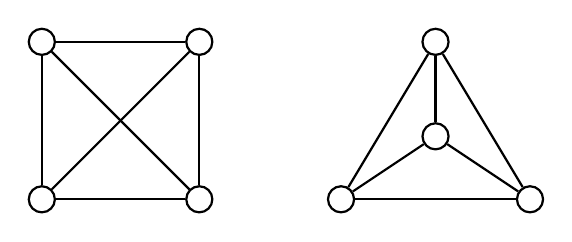
\begin{tikzpicture}
    \begin{scope}[every node/.style={circle,thick,draw}]
        \node (1) at (-1,-1) {};
        \node (2) at (-1,1) {};
        \node (3) at (1,1) {};
        \node (4) at (1,-1) {};
    \end{scope}
    
    \path[-,draw,thick] 
        (1) edge (2)
        (1) edge (3)
        (1) edge (4)
        (2) edge (3)
        (2) edge (4)
        (3) edge (4);
    
    \begin{scope}[xshift=4cm, every node/.style={circle,thick,draw}]
        \node (5) at (0,-0.2) {};
        \node (6) at (-1.2,-1) {};
        \node (7) at (1.2,-1) {};
        \node (8) at (0, 1) {};
        \path[-,draw,thick]
            (5) edge (6)
            (5) edge (7)
            (5) edge (8)
            (6) edge (7)
            (6) edge (8)
            (7) edge (8);
    \end{scope}
    \end{tikzpicture}

    \caption{Ravninskost grafa $K_4$ ni očitna.}
\end{figure}

Hitro lahko vidimo, da grafa $K_5$ in $K_{3,3}$ nista ravninska (poskusimo ju narisati v ravnini, a kmalu ugotovimo, da to ne bo mogoče). To dejstvo sledi tudi kot posledica ene izmed posledic Eulerjeve formule.

Spomnimo se, da je risba grafa predstavitev grafa v ravnini, pri čemer vozlišča ustrezajo točkam v ravnini, povezave pa enostavnim krivuljam med točkami. Te točke in enostavne krivulje lahko ravnino razdelijo na več delov -- takim območjem pravimo \emph{lica vložitve}. Lice, ki je neomejeno in obdaja celotno risbo grafa, je \emph{zunanje}.

\begin{figure}[h]
    \caption{Zunanje lice grafa.}
\end{figure}

\begin{izrek}[Eulerjeva formula]
    \label{izr:euler-formula}
    Naj bo $G$ povezan ravninski graf z $n$ vozlišči in $m$ povezavami. Naj ima risba grafa $G$, vloženega v ravnino, $f$ lic. Potem velja
    \[ n - m + f = 2 .\]
\end{izrek}

Za dokaz Eulerjeve formule bomo potrebovali še definicijo drevesa:

\begin{definicija}
    \emph{Drevo} je povezan graf brez ciklov.
\end{definicija}

Vidimo lahko, da risba drevesa premore le eno lice -- zunanje.

\begin{figure}[h]
    \caption{Drevo na 7 vozliščih.}
\end{figure}

Za vsako drevo z vsaj dvema vozliščema velja, da vsebuje vozlišče stopnje 1 -- takemu vozlišču v drevesu pravimo \emph{list} -- saj bi v nasprotnem primeru graf vseboval neskončno pot ali cikel. Za drevesa velja tudi:

\begin{lema}
    Če je T drevo z $n$ vozlišči in $m$ povezavami, je $m=n-1$.
\end{lema}

\begin{proof}
    Lemo bomo dokazali z indukcijo na število vozlišč.
    
    Baza indukcije: Če ima drevo le eno vozlišče, nima nobene povezave (velja $n = 1$ $m = 0 = n-1$).
    
    Indukcijska predpostavka: Drevo z $n-1$ vozlišči ima $n-2$ povezav.
    
    Indukcijski korak: Vzamemo drevo z $n$ vozlišči in $m$ povezavami. Vemo ($n \geq 2$), da vsebuje vsaj en list -- označimo ga z $x$. Če $x$ odstranimo iz grafa, dobimo novo drevo z $n-1$ vozlišči in $m-1$ povezavami, saj je bilo vozlišče $x$ stopnje 1. Po indukcijski predpostavki za novo drevo velja:
    \begin{align*}
        (m-1) &= (n-1) - 1 \\
        m     &= n - 1 \qedhere
    \end{align*}
\end{proof}

Če želimo, da velja tudi obratno, pa moramo zahtevati še, da je graf povezan. Graf je torej drevo natanko tedaj, ko je povezan in je število njegovih povezav $m$ enako $n-1$. Dokaz tega dejstva je naveden v~\cite[str.~57]{bib:potocnik}.

\begin{proof}[Dokaz izreka~\ref{izr:euler-formula}]
    Formulo dokažemo z indukcijo na število povezav.
    
    Naj bo $m = n-1$. Imamo torej drevo, za katerega vemo, da njegova risba premore le zunanje lice, $f$ je torej enak 1. Sledi
    \[ n - (n-1) + 1 = 2. \]
    
    Predpostavimo, da formula velja za vsak graf na $n$ vozliščih in $m-1$ povezavah.
    
    Če sedaj vzamemo graf $G$ z $m \geq n$ povezavami, graf torej vsebuje vsaj en cikel. Izberimo nek cikel v grafu in ga označimo s $C$, lice, ki ga ta cikel omejuje, pa označimo z $F$. Če iz grafa odstranimo eno od povezav $e$ cikla $C$, nimamo več cikla, zato preostanek $C \setminus e$ ne omejuje več tega lica. Označimo $G' = G \setminus e$. $G'$ ima še vedno $n'=n$ vozlišč, a eno povezavo in lice manj kot prej ($m'=m-1$, $f'=f-1$). Po indukcijski predpostavki sledi
    
    \begin{align*}
        n' - m' + f'      &= 2 \\
        n - (m-1) + (f-1) &= 2 \\
        n - m + f         &= 2 \qedhere
    \end{align*}
\end{proof}

Naslednja posledica Eulerjeve formule nam bo pomagala pri dokazu dejstva, da grafa $K_5$ in $K_{3,3}$ nista ravninska.

\begin{posledica}
    Če je $G$ ravninski graf na $n$ vozliščih in $m$ povezavah, velja
    \begin{equation} 
    \label{eq:posledica-euler-formula}
    m \leq 3n - 6.
    \end{equation}
    Če $G$ ne vsebuje trikotnikov, pa velja formula
    \begin{equation} 
    \label{eq:posledica-euler-formula-trik}
    m \leq 2n - 4.
    \end{equation}
\end{posledica}

\begin{proof}
    Če za vsako lice upoštevamo le tri povezave (to je minimalno število povezav, ki omejujejo lice, ki ni zunanje), bomo dobili kvečjemu manj, kot če preštejemo vse povezave dvakrat.
    Vsaka povezava namreč omejuje največ dve lici; če bi po vseh licih sešteli število povezav, ki omejujejo neko lice, bi torej dobili dvakratno vrednost števila povezav.
    Torej velja neenakost
    \[ 3f \leq 2m .\]
    Če iz Eulerjeve formule izrazimo $f$ in ga vstavimo v zgornjo neenakost, dobimo
    \begin{align*}
        3\cdot(2-n+m) &\leq 2m \\
        6 - 3n + 3m &\leq 2m \\
        m &\leq 3n - 6
    \end{align*}
    
    Na podoben način pokažemo formulo~\eqref{eq:posledica-euler-formula-trik}, le da začnemo z neenakostjo 
    \[ 4f \leq 2m, \]
    saj je zaradi predpostavke, da graf ne vsebuje trikotnikov, minimalno število povezav, ki omejuje lice, enako 4. 
\end{proof}

Z uporabo zgornje formule, ki torej mora veljati, če je graf ravninski, lahko dokažemo:
\begin{posledica}
    \label{posl:neravninska-grafa}
    $K_5$ in $K_{3,3}$ nista ravninska grafa.
\end{posledica}

\begin{proof}
    Polni graf na petih vozliščih $K_5$ ima {$5 \choose 2$} = 10 povezav. $n$ je torej v tem primeru enak
    5, $m$ pa je 10. Če bi bil $K_5$ ravninski, bi morala veljati formula~\eqref{eq:posledica-euler-formula},
    a temu ni tako:
    \[ 10 = m \nleq 3n - 6 = 9 \]
    Torej $K_5$ ni ravninski.
    
    Podobno lahko pokažemo tudi za poln dvodelni graf $K_{3,3}$, pri čemer je $n$ enak 6, število povezav $m$ pa 9. Če bi bil ta graf ravninski, bi morala veljati formula~\eqref{eq:posledica-euler-formula-trik}, a to ne drži:
    \[ 9 = m \nleq 2n - 4 = 8. \] 
    Graf $K_{3,3}$ torej ni ravninski. \qedhere
\end{proof}

Sedaj želimo ugotoviti, kakšnim pogojem mora ustrezati graf, da bo ravninski. Očitno velja naslednja trditev:

\begin{trditev}
    \label{trd:podgraf}
    Če je graf ravninski, potem je tudi vsak njegov podgraf ravninski. %\cite{bib:potocnik}
\end{trditev}

Operacija ``podgraf'' torej ohranja ravninskost grafa.
Pogledali si bomo še operacijo \emph{subdivizije}, ki prav tako ohranja lastnost ravninskosti. Če vzamemo neko povezavo $e$ grafa $G$ in na sredino te povezave dodamo še eno vozlišče (v ravnini ga predstavlja točka), na tak način dobimo nov graf z operacijo subdivizije. \cite[str.~66]{bib:potocnik}

\begin{definicija}
    Graf $H$ je \emph{subdivizija} grafa $G$, če ga lahko dobimo iz $G$ z zaporednim \emph{subdiviziranjem} povezav grafa $G$.\cite[str.~66]{bib:potocnik}
\end{definicija}

Iz definicije je razvidno, da je tak $H$ ravninski natanko tedaj, ko je $G$ ravninski. Iz tega dejstva, trditve~\ref{trd:podgraf} in posledice~\ref{posl:neravninska-grafa} lahko zaključimo, da graf zagotovo ni ravninski, če vsebuje subdivizijo $K_5$ ali $K_{3,3}$. Zanimivo pa je, da velja tudi obratno; dokaz tega dejstva je netrivialen in ga lahko najdemo v [TODO vir].

\begin{izrek}[Kuratowski]
    \label{izr:kuratowski}
    Graf G je ravninski natanko tedaj, ko ne vsebuje subdivizije $K_5$ niti subdivizije $K_{3,3}$.
\end{izrek}
%\begin{definicija}
%	\emph{Barvanje} grafa $\graf$ je preslikava 
%	\[ c\colon \vozlisca \to \N, \text{ tako da velja } av \in \povezave \implies c(a) \neq c(v). \]
%	Če je $c\colon \vozlisca \to [k]$, rečemo, da je $c$ $k$-barvanje. \emph{Kromatično število} grafa $G$, $\mathcal{X}(G)$, je najmanjši $k$, za katerega obstaja $k$-barvanje grafa G.
%\end{definicija}

\section{Klasični problem londonskega stolpa}
Pri klasičnem londonskem stolpu imamo tri enako velike krogle različnih barv in tri palice različnih velikosti: na prvo lahko postavimo eno kroglo, na drugo dve, na tretjo pa tri (temu bomo rekli, da imajo palice višine 1, 2 in 3). Cilj igre je priti iz nekega začetnega stanja v neko vnaprej določeno končno stanje.

\begin{figure}[h]
    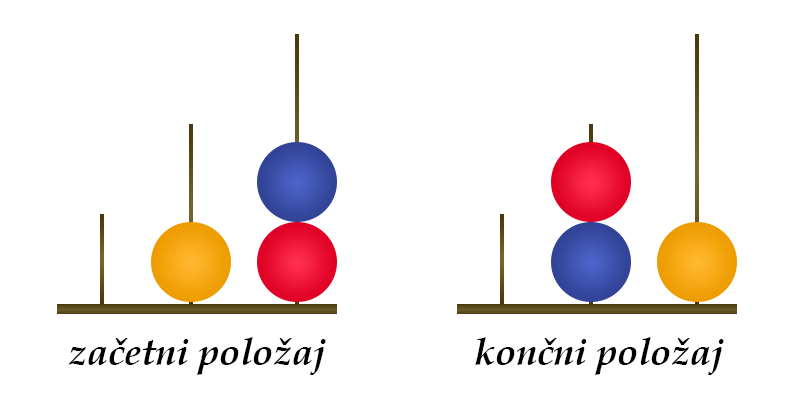
\includegraphics[width=250pt]{img/london-tower.png}
    \caption{Na sliki sta prikazani dve možni stanji londonskega stolpa.}
    \label{fig:stanji}
\end{figure}

Stanja in prehode med njimi si najlažje predstavljamo, če narišemo graf. V ta namen vpeljemo naslednje oznake:
krogle bomo označili s številkami 1, 2, 3 -- npr.\ modra krogla naj ima oznako 1, rdeča 2, rumena pa 3 -- s simbolom ``|'' pa bomo označili konec prejšnje palice in začetek nove. Krogle bomo naštevali od vrha palice navzdol.

\begin{primer}
    Začetno stanje na sliki~\ref{fig:stanji} lahko torej opišemo z $\bd 3 \ed 12$, končno stanje pa z $\bd 21 \ed 3$.
\end{primer}
\medskip

S pomočjo teh oznak lahko opišemo vsako možno stanje in narišemo graf londonskega stolpa (označimo ga z $L$), pri čemer so vozlišča stanja, povezave pa so med tistimi stanji, med katerimi lahko prehajamo z eno potezo (enim veljavnim premikom krogle).

\begin{figure}[h!]
    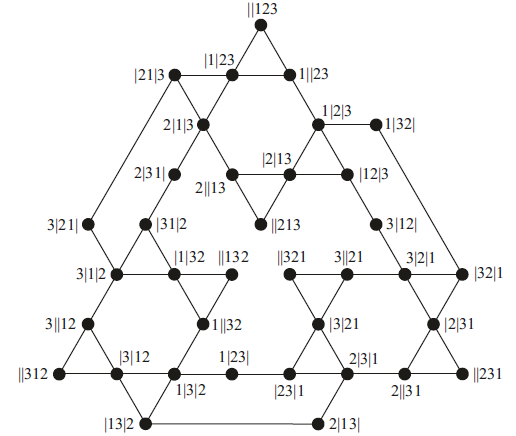
\includegraphics[width=300pt]{img/tolgraph.png}
    \caption{Graf $L$ klasičnega Londonskega stolpa.}
    \label{fig:tolgraph}
\end{figure}

\begin{lema}
    \label{lem:stanja-klas-lond}
    Število vseh možnih stanj klasičnega londonskega stolpa je 36.
\end{lema}

\begin{proof}
    Najprej si oglejmo vse možne postavitve krogel, pri čemer se ne oziramo na barvo.
    Imamo dve možnosti:
    \begin{enumerate}
        \item \textbf{Na prvi (najkrajši) palici je krogla.}
        Preostali dve krogli lahko razdelimo na drugi dve palici tako, da:
        \begin{itemize}[label={-}]
            \item je prazna druga palica,
            \item je prazna tretja palica,
            \item ima vsaka palica po eno kroglo.
        \end{itemize}
        Torej imamo v tem primeru tri možnosti.
        
        \item \textbf{Na prvi (najkrajši) palici ni krogle.}
        Na drugi dve palici moramo torej razdeliti vse tri krogle.
        Ponovno imamo tri možnosti:
        \begin{itemize}[label={-}]
            \item druga palica je prazna, tretja palica pa polna (na njej so tri krogle),
            \item na drugi palici je ena krogla, na tretji palici pa dve krogli,
            \item druga palica je polna (na njej sta dve krogli), na tretji palici pa je ena krogla.
        \end{itemize}
    \end{enumerate}
    Po pravilu vsote imamo torej, če se ne oziramo na barve krogel, $3+3=6$ možnih postavitev krogel.
    V vsaki od teh lahko še premešamo barve krogel, torej imamo za vsako postavitev $3!$ možnosti. Sledi, da je vseh možnih stanj $3! \cdot 6 = 6 \cdot 6 = 36$.\qedhere
\end{proof}

Iz leme~\ref{lem:stanja-klas-lond} sledi, da ima $L$ ima 36 vozlišč. Graf je ravninski, saj je na sliki~\ref{fig:tolgraph} narisan v ravnini brez križanja povezav. Hitro vidimo, da je 12 vozlišč grafa $L$ stopnje 2, drugih 12 je stopnje 3, zadnjih 12 pa stopnje 4. Preverimo lahko tudi, da je premer klasičnega londonskega grafa enak 8.

\begin{primer}
    S pomočjo grafa na sliki~\ref{fig:tolgraph} lahko hitro ugotovimo, da za prehod med stanjema na sliki~\ref{fig:stanji} potrebujemo minimalno 4 poteze in da je to edino najkrajše možno zaporedje potez.
\end{primer}

\bigskip

\begin{trditev}
    Graf $L$ vsebuje Hamiltonovo pot, ne pa tudi Hamiltonovega cikla.
\end{trditev}

\begin{proof}
    TODO
    
    Hitro lahko dokažemo, da $L$ vsebuje Hamiltonovo pot: poiščemo jo. Ena izmed Hamiltonovih poti v grafu $L$ je prikazana na sliki~\ref{}.
    
    Da bi dokazali, da graf ni Hamiltonov, moramo najprej opaziti nekaj lastnosti tega grafa. Soseščina vsakega vozlišča stopnje 2 je sestavljena iz enega vozlišča stopnje 3 in enega stopnje 4, prav tako je presek soseščin poljubnih dveh vozlišč stopnje 2 prazen -- vsako vozlišče stopnje 2 ima torej ``svoje'' vozlišče stopnje 3 in stopnje 4. Nadalje lahko iz grafa vidimo, da poljubni dve vozlišči stopnje 3 nista sosednji.
    
    Sledi, da na ciklu $C$ v grafu, ki bi vseboval vsa vozlišča, nobeni dve vozlišči stopnje 4 nista sosednji. Ker imamo po 12 vozlišč vsake stopnje, bi v nasprotnem primeru namreč prišli do zaključka, da morata biti sosednji dve vozlišči stopnje 3, kar pa je v protislovju z zgornjim opažanjem.
    
    Sedaj začnimo graditi cikel $C$, ki bo vseboval vsa vozlišča grafa natanko enkrat. Oglejmo si sliko~\ref{}.
    Cikel $C$ mora torej gotovo iti skozi vsa vozlišča stopnje 2, kar je možno le na en način: če imamo vozlišče stopnje 2 $v$ s sosedoma $u$ stopnje 3 in $z$ stopnje 4, mora $C$ vsebovati pot $u,v,z$.
    Če začnemo pri vozlišču stopnje 2 $||\,123$, mora graf torej vsebovati pot $1||23, ||123, |1|23$. Slednje je vozlišče stopnje 4, za nadaljevanje cikla pa imamo dve možnosti: vozlišče $2|1|3$ ali $|21|3$. Ker je prvo stopnje 4 in smo že prej opazili, da dve vozlišči iste stopnje ne bosta sosednji na ciklu $C$, cikel nadaljujemo z $|21|3$. Sosed tega vozlišča je vozlišče $3|21|$ stopnje 2, zato moramo cikel gotovo nadaljevati skozi njega. Pridemo do vozlišča $3|1|2$. Imamo dve možnosti: 
    \begin{itemize}[label={-}]
        \item Nadaljujemo z vozliščem $|31|2$, ki je stopnje 3 in je na notranjem ciklu. V tem primeru ne bomo notranjega cikla nikoli zapustili, saj je notranji cikel oblike: vozlišče stopnje 2, vozlišče stopnje 3 (povezano samo z vozlišči na notranjem ciklu), vozlišče stopnje 4, ki je nato povezano z vozliščem stopnje 2, skozi katerega moramo iti. Nato pa sledita vozlišče $a$ stopnje 3 (povezano z notranjim ciklom in vozliščem stopnje $w$ 4 na zunanjem ciklu) in vozlišče $b$ stopnje 4 (povezan z vozliščem $c$ stopnje 2 in še dvema drugima na notranjem ciklu ter vozliščem $w$). Ker moramo iti skozi vozlišče $c$, moramo tudi skozi $b$, od prej pa vemo, da moramo nujno tudi skozi $a$, saj je sosed vozlišča stopnje 2. Torej lahko pot speljemo le skozi $a,b,c$, saj je $w$ stopnje 4 in na ciklu zato ne sme biti soseden $b$, ki je prav tako stopnje 4.
        \item Pot torej nadaljujemo z vozliščem stopnje 3 na zunanjem ciklu $3||12$, in tudi v nadaljevanju ostanemo na zunanjem ciklu, saj vemo, da bomo v nasprotnem primeru ostali na notranjem ciklu.
    \end{itemize}
    Torej ne moremo konstruirati cikla, bi vseboval vsa vozlišča našega grafa $L$ natanko enkrat. $L$ torej ni Hamiltonov.
    \qedhere
\end{proof}

\section{Posplošeni londonski stolp}
Graf klasičnega problema londonskega stolpa je majhen, zato je za psihološka testiranja naloga včasih prelahka. 
Jenny R. Tunstall je prva predlagala razširitev klasičnega londonskega stolpa na 4 krogle s podaljšanimi palicami (vsaka je podaljšana za eno enoto), mi pa si bomo v tem razdelku pogledali ta problem v splošnem, s $p \geq 3$ palicami in $n \geq 2$ kroglami.

\subsection{Definicija}

Posplošen londonski stolp ima $n \geq 2$ krogel, označimo jih s številkami $1,\ldots,n$, in $p \geq 3$ palic, katerih višino označimo s $h_k$ -- toliko krogel lahko postavimo na $k$-to palico. Seveda velja, da mora biti število vseh krogel manjše ali enako vsoti višin vseh palic, sicer vseh krogel ne moremo razporediti na palice. Veljati mora torej:
\[ n \leq \sum_{k=1}^{p} h_k.\]
Edina omejitev premikov krogel je ponovno višina palic, prav tako je enak cilj igre, priti iz začetnega stanja v končno stanje s čim manj premiki.

Še pred definicijo splošnega londonskega grafa vpeljimo oznake, ki jih bomo uporabljali za opis stanja nekega posplošenega londonskega stolpa. Enoličen zapis lahko dosežemo, če vsako stanje predstavimo s permutacijo $s$ iz simetrijske grupe $S_{n+p}$. Pri tem $i$-ta števka permutacije predstavlja

\[ s_i =
\begin{cases}
    \text{položaj krogle } i, & i \in [n] \\
    \text{položaj dna palice } i-n, & i \in [n+p] \setminus [n]
\end{cases}
\]

Položaje oštevilčimo od leve palice proti desni, z vrha palice proti dnu. Tako bo s številko 1 oštevilčen položaj krogle, ki je postavljena najvišje na prvi palici; če na prvi palici ni nobene krogle, bo imelo položaj 1 dno te palice.

\begin{primer}
    Poiščimo permutacijo za začetni položaj na sliki~\ref{fig:stanji}, ki smo ga označili z $|3|12|$. 
    Predstavljajmo si, da oštevilčujemo krogle in dna palice, in začnimo oštevilčevati od leve proti desni, z vrha palice proti dnu, tako kot je prikazano na sliki~\ref{fig:ostev-stanji}.
    
    \begin{figure}[h]
        \caption{Položaji krogel in palic za stanje $|3|12|$.}
        \label{fig:ostev-stanji}
    \end{figure}
    
    Sedaj le preberemo položaje vseh krogel (od prve do tretje) in vseh palic (od leve proti desni) -- prva (modra) krogla je oštevilčena s 4, druga (rdeča) s 5, \ldots
    To stanje lahko torej predstavimo s permutacijo $s=452136$.
\end{primer}

Hitro vidimo, da mora veljati 
\[\forall k \in [p]\colon s_{n+k} - s_{n+k-1} \geq 1 \]
saj je $s_{n+k}$ položaj dna palice $k$, $s_{n+k-1}$ pa položaj dna palice $k-1$, torej se mora njun položaj razlikovati najmanj za 1 -- to se zgodi, če na palici $k$ ni nobene krogle.

Prav tako pa mora veljati tudi 
\[\forall k \in [p]\colon s_{n+k} - s_{n+k-1} \leq h_k + 1,\]
kar se zgodi v primeru, če je na $k$-ti palici $h_k$ krogel.

Opazimo še, da je položaj dna zadnje palice, $s_{n+p}$, vedno enak $n+p$, saj smo pred tem že oštevilčili položaje vseh $n$ krogel in ostalih $p-1$ palic.

V splošnem je londonski graf, katerega vozlišča so vsa stanja pripadajočega londonskega stolpa, torej smiselno definirati takole:

\begin{definicija}
    Za \emph{londonski graf} $L_h^n$, kjer je $p \geq 3,\ n \geq 2,\ h \in [n]^p,\  \sum_{k=1}^p h_k \geq n$ velja:
    \begin{itemize}
        \item vozlišča so vse permutacije $s \in S_{n+p}$, za katere velja:
        \[\forall k \in [p]:\ 1 \leq s_{n+k} - s_{n+k-1} \leq h_k + 1,\ s_{n+p} = n + p ,\]
        \item vsaki dve stanji (oz.\ pripadajoči permutaciji), med katerima lahko prehajamo z veljavno potezo, sta povezani.
    \end{itemize}
\end{definicija}

S pogojem, da so vse palice visoke največ $n$, ne izgubimo splošnosti, saj razporejamo le $n$ krogel.

Očitno je klasičen londonski graf $L$ enak $L_{123}^3$, saj imamo 3 krogle in 3 palice, ki so velikosti 1, 2 in 3.
Če smo v tem primeru lahko izračunali število vozlišč, pa je v splošnem za londonske stolpe to precej težko. V naslednjem podrazdelku bomo obravnavali poseben primer londonskih grafov, za katerega je znana formula za število vozlišč. 

\subsection{Oxfordski graf}

\emph{Oxfordski graf} je poseben primer londonskega grafa, za katerega velja, da so vse palice velikosti $n$, pri čemer je $n$ število krogel. Oxfordski graf označimo z $O^n_p$, zanj torej velja $O^n_p := L^n_{n^p}$.

Medtem ko je v splošnem težko določiti število vozlišč londonskega grafa, pa je to precej bolj preprosto za oxfordski graf. Še več, določimo lahko tudi število povezav.

\begin{trditev}
    Število vozlišč oxfordskega grafa $O^n_p$ je enako 
    \begin{equation}
        \label{eq:oxford-vozl}
        \frac{(n+p-1)!}{(p-1)!}.
    \end{equation}

\end{trditev}

\begin{proof}
    Iščemo število vseh možnih stanj krogel oxfordskega stolpa, saj je to enako številu vozlišč oxfordskega grafa.
    Podobno kot pri dokazu števila stanj klasičnega londonskega stolpa najprej pozabimo na različne barve krogel (pretvarjamo se, da so krogle enake) in se osredotočimo samo na njihovo postavitev. 
    
    Na koliko načinov lahko $n$ enakih krogel razporedimo na $p$ palic višine $n$? Pri tem nimamo nobenih omejitev, saj so palice dovolj visoke, da lahko vse krogle postavimo tudi na eno samo palico. Lahko si predstavljamo, da imamo vse krogle zložene v vrsto, označene naj bodo z 0, nato pa na poljubna mesta (s ponavljanjem) vrivamo 1, ki naj pomeni konec neke palice in začetek neke druge. Ko vrinemo $p-1$ enic, smo določili $p$ palic in s tem razporeditev krogel. 
    
    Sedaj lahko na problem pogledamo malo drugače: na $n+p-1$ mest razporejamo $n$ ničel, ki predstavljajo krogle, in $p-1$ enic, ki predstavljajo začetek nove palice. Če razporedimo vse enice, bodo vsa preostala mesta zasedle ničle, razporeditev bo s tem točno določena. Načinov za izbiro $p-1$ mest za enice izmed $n+p-1$ položajev je ${n+p-1 \choose p-1}$. Če privzamemo, da so vse krogle enake, je vseh možnih razporeditev torej ${n+p-1 \choose p-1}$.
    
    Ker je vsaka krogla drugačne barve, imamo za vsako razporeditev še $n!$ možnih permutacij barv. Število vseh stanj, in zato tudi število vozlišč, je tako enako
    
    \[ n! \cdot {n+p-1 \choose p-1} = n! \cdot \frac{(n+p-1)!}{n!(p-1)!} = \frac{(n+p-1)!}{(p-1)!}. \] \qedhere
\end{proof}

\begin{trditev}
    Število povezav oxfordskega grafa $O^n_p$ je enako
    \begin{equation}
        \label{eq:povezave-oxf}
        \frac{np}{2} \frac{(p-2+n)!}{(p-2)!}
    \end{equation}
    \label{trd:povezave-oxf}
\end{trditev}

Preden si ogledamo izpeljavo formule~\eqref{eq:povezave-oxf}, pa si na hitro oglejmo še sledečo lemo, ki jo bomo potrebovali pri dokazu.

\begin{lema}
    Velja naslednja lastnost binomskih simbolov:
    \begin{equation}
        \label{eq:binom}
        {b+w \choose l} = \sum_{k=0}^{l}{b \choose k}{w \choose l-k}.
    \end{equation}
\end{lema}

\begin{proof}
    Formulo najlažje dokažemo kombinatorično. Predstavljajmo si, da imamo v posodi $b$ črnih in $w$ belih krogel, iz posode pa izbiramo $l$ krogel.
    
    Leva stran enakosti nam predstavlja vse možne načine izbire $l$ krogel izmed $b+w$ krogel (brez vračanja). 
    
    Na to pa lahko gledamo tudi malo drugače: najprej določimo neko fiksno število $k$, toliko krogel bomo izbrali izmed črnih, preostanek pa bomo izbrali iz belih krogel. Za fiksen $k$ je število možnih izbir ravno ${b \choose k}{w \choose l-k}$. Če to sedaj seštejemo po vseh možnih $k$-jih, bomo dobili ravno vse možne načine izbire $l$ krogel izmed $b+w$ krogel, formula~\eqref{eq:binom} torej velja.
\end{proof}

\begin{proof}[Dokaz trditve~\ref{trd:povezave-oxf}]
    Vzemimo stanje (vozlišče), pri katerem je $q$ palic nepraznih, $1 \leq q \leq p$ in $n \geq q$. Vsako vrhnjo kroglo ene izmed $q$ palic lahko premaknemo na katerokoli palico, razen trenutne; izberemo torej eno izmed $q$ palic, s katere premaknemo kroglo, in eno izmed preostalih $p-1$ palic, kamor kroglo premaknemo. Tako vozlišče je torej stopnje $q(p-1)$. (Pri tem upoštevamo, da je povezava med dvema vozliščema grafa pravzaprav veljavna poteza med dvema stanjema.)
    
    Vseh stanj, ki imajo točno $q$ nepraznih palic, je enako
    \[{p \choose q} \frac{n!}{(n-q)!} \cdot |V(O^{n-q}_q)|.\]
    Najprej izberemo $q$ izmed $p$ palic, ki bodo neprazne, kar lahko storimo na ${p \choose q}$ načinov. Na vsako izmed teh $q$ palic moramo nujno postaviti vsaj eno kroglo, kar lahko naredimo na $n \cdot (n-1) \cdot \ldots \cdot (n-q+1) = \frac{n!}{(n-q)!}$ (za prvo izmed $q$ palic imamo na voljo $n$ krogel, za drugo $n-1$ krogel,\ldots). Preostalih $n-q$ krogel pa lahko razporedimo poljubno na $q$ palic, kar je brez škode za splošnost enako številu razporeditev $n-q$ krogel na $q$ palic velikosti $n-q$, torej $|V(O^{n-q}_q)|$.
    Če uporabimo formulo za število vozlišč oxfordskega grafa~\eqref{eq:oxford-vozl} in poračunamo, dobimo, da je število takih stanj enako
    \begin{align*}
        {p \choose q} \frac{n!}{(n-q)!} \cdot |V(O^{n-q}_q)| &=
        {p \choose q} \frac{n!}{(n-q)!} \frac{(n-q+q-1)!}{(q-1)!} \\ &= n! {p \choose q} \frac{(n-1)!}{(q-1)!\,(n-q)!} \\ &=
        n! {p \choose q} {n-1 \choose q-1}
    \end{align*}

    Sedaj po $q$ seštejemo stopnje vseh vozlišč (upoštevamo, da imajo vsa vozlišča, kjer je nepraznih točno $q$ palic, enako stopnjo) in uporabimo formulo~\eqref{eq:lema-o-rokovanju} iz leme o rokovanju:
    \begin{align*}
        |E(O^n_p)|
        &= \frac{1}{2} \sum_{q=1}^{p} \overbrace{q(p-1)}^{\text{stopnja vozlišča}} 
        \overbrace{n! {p \choose q} {n-1 \choose q-1} }^{\text{št.~vozlišč s to stopnjo}} \\
        &= \frac{1}{2} (p-1) n! \sum_{q=1}^{p} q {p \choose q} {n-1 \choose q-1} \\
        &= \frac{1}{2} (p-1) n! \sum_{q=1}^{p} q \frac{p!}{q! \, (p-q)!} {n-1 \choose q-1} \\
        &= \frac{1}{2} (p-1) n! \sum_{q=1}^{p} p \frac{(p-1)!}{(q-1)! \, (p-q)!} {n-1 \choose q-1} \\
        &= \frac{1}{2} p (p-1) n! \sum_{q=1}^{p} {p-1 \choose q-1} {n-1 \choose q-1}
    \end{align*}
    Sedaj uvedemo nov indeks $k = q-1$, upoštevamo lastnosti binomskih simbolov in uporabimo zgoraj dokazano formulo~\eqref{eq:binom}:
    \begin{align*}
        |E(O^n_p)|
        &= \frac{1}{2} p (p-1) n! \sum_{k=0}^{p-1} {p-1 \choose k} {n-1 \choose k} \\
        &= \frac{1}{2} p (p-1) n! \sum_{k=0}^{p-1} {p-1 \choose p-1-k} {n-1 \choose k} \\
        &= \frac{1}{2} p (p-1) n! {p-1 + n-1 \choose p-1} \\
        &= \frac{1}{2} p (p-1) n! {n + p - 2 \choose p-1} \\
        &= \frac{1}{2} p (p-1) n! \frac{(n+p-2)!}{(p-1)!\,(n-1)!} \\
        &= \frac{1}{2} p n \frac{(n+p-2)!}{(p-2)!} \\
        &= \frac{np}{2} \frac{(p-2+n)!}{(p-2)!} \qedhere
    \end{align*}
\end{proof}

\subsection{Povezanost}

Zaželjeno je, da lahko pri londonskem stolpu, s pomočjo katerega opravljajo teste v psihologiji, prehajamo med poljubnima dvema stanjema. To velja, če je pripadajoči londonski graf povezan, kar je zato ena pomembnejših lastnosti tega grafa.
V nadaljevanju bomo privzeli, da so palice urejene po velikosti naraščajoče, velja torej $h_1 \leq h_2 \leq \cdots \leq h_p$.
Potreben pogoj za povezanost londonskega grafa je očitno 
\[ n \leq \sum_{k=1}^{p-1} h_k, \]
oziroma z besedami, da lahko krogle razporedimo tako, da najvišja palica ostane prazna. V nasprotnem primeru bi, po tem ko bi razporedili maksimalno možno število krogel na vse preostale (manjše) palice, na največji ostalo še nekaj krogel, ki jih nikoli ne bi mogli premakniti na kakšno drugo palico.
Izkaže se, da je ta pogoj tudi zadosten za povezanost londonskega grafa.

\begin{izrek}
    Londonski graf $L_h^n$ je povezan natanko tedaj, ko velja pogoj
    \begin{equation}
        n \leq \sum_{k=1}^{p-1} h_k.
        \label{eq:pogoj-povezanosti}
    \end{equation}
\end{izrek}

\begin{proof}
    Želimo dokazati, da iz pogoja \eqref{eq:pogoj-povezanosti} sledi, da lahko najdemo pot med poljubnima dvema vozliščema v londonskem grafu, kar je ravno definicija povezanosti. Dokaza se lotimo tako, da najprej čim bolj zreduciramo splošen problem in nato rešimo zreduciran problem.
    
    Spomnimo se, da vsako vozlišče londonskega grafa predstavlja neko stanje krogel -- če torej iščemo pot v grafu med dvema vozliščema, pravzaprav rešujemo problem, kako iz začetnega stanja krogel priti v končno. Fiksirajmo poljubno začetno in končno stanje in poskusimo rešiti ta problem.
    
    Predpostavili bomo, da je število vseh krogel kar enako vsoti višin vseh palic brez največje, saj lahko v nasprotnem primeru vpeljemo navidezne krogle, katerih premike kasneje zanemarimo. Velja naj torej $n = \sum_{k=1}^{p-1}h_k$.
    
    Nadalje lahko predpostavimo, da so krogle pri začetnem kot tudi pri končnem stanju razporejene tako, da je največja palica prazna. V nasprotnem primeru jih lahko na začetku razporedimo na preostale palice, na koncu pa preprosto prestavimo na največjo palico.

    Torej je za dokaz povezanosti grafa dovolj, če najdemo pot med poljubnima dvema stanjema, pri katerem so vse palice (razen največje) zapolnjene, največja palica pa je prazna.
    
    Sedaj postopamo tako, da izberemo kroglo, ki še ni na svojem (končnem) položaju, in jo zamenjamo s kroglo, ki se trenutno nahaja na tem položaju; ta postopek ponavljamo. Če lahko zamenjavo naredimo tako, da se pri tem ne spremeni položaj nobene druge krogle, je po koncu zamenjave še ena krogla več na pravem mestu.
    Ker je največja palica prazna, vse druge pa zapolnjene, se po koncu ponavljanja tega postopka ne more zgoditi, da je le ena krogla (označimo jo z $a$) na napačnem mestu. V nasprotnem primeru bi zaradi zapolnjenosti palic namreč obstajala krogla $b$, ki bi bila na končnem mestu krogle $a$ in zato $b$ ne bi bila na svojem končnem položaju -- torej imamo vedno vsaj dve krogli, ki sta na napačnem mestu, ti dve krogli pa lahko spet zamenjamo.
    
    Če torej dokažemo, da lahko poljubni dve krogli zamenjamo tako, da se pri tem ne spremeni položaj nobene druge krogle, bomo s ponavaljanjem zgornjega postopka lahko prešli iz začetnega v končno stanje krogel, graf bo povezan.
    
    Sedaj predpostavimo še, da je ena izmed krogel, ki ju bomo zamenjali, na vrhu prve, najmanjše, palice. Namreč, s tremi zamenjavami, pri katerih je ena izmed krogel vedno na vrhu prve palice, lahko nadomestimo splošno zamenjavo dveh poljubnih krogel. Recimo, da želimo zamenjati poljubni krogli $a$ in $b$. Če uporabimo notacijo klasičnega problema, s $c$ označimo vrhnjo kroglo prve palice, z $x$ pa poljubno število nekih poljubnih krogel in če izpustimo palice, ki na to menjavo ne bodo imele vpliva, lahko menjavo $a$ in $b$ opravimo takole:
    
    \[ cx|xax|xbx| \rightarrow bx|xax|xcx| \rightarrow ax|xbx|xcx| \rightarrow cx|xbx|xax|. \]
    
    Pri tem je bila v vsaki menjavi udeležena vrhnja krogla prve palice.
    Dovolj je torej dokazati, da lahko naredimo menjavo vrhnje krogle prve palice in neke druge poljubne krogle, brez da bi pri tem pokvarili položaj ostalih krogel.
    
    Sedaj si izberimo kroglo, ki ni na pravem položaju, in s tem tudi kroglo, ki je trenutno na njenem položaju. Predpostavili smo, da je ena izmed teh krogel na prvi palici -- to kroglo označimo z $a$, drugo pa z $b$. Ločimo dva primera:
    
    \begin{enumerate}
        \item \textbf{Krogla $b$ je na prvi palici.}
        Vrhnjo kroglo druge palice, označimo jo s $c$, premaknemo na največjo ($p$-to) palico. Nato kroglo $a$ premaknemo na vrh druge palice, preostale krogle na prvi palici z do vključno kroglo $b$ pa premaknemo (seveda eno naenkrat) na največjo palico. Krogla $a$ lahko sedaj zasede svoj pravi položaj na prvi palici, $b$ pa premaknemo iz vrha največje palice na vrh druge. Sedaj lahko vrnemo vse preostale krogle (razen $c$) na prejšnje mesto na prvi palici, nato lahko na vrh prve palice postavimo $b$, ki tako zavzame prejšnji položaj krogle $a$. Za konec premaknemo še kroglo $c$ z največje palice na vrh druge palice.
        \item \textbf{Krogla $b$ ni na prvi palici.}
        V tem primeru je postopek še nekoliko lažji: najprej vse krogle nad $b$ premaknemo na največjo palico, nato na vrh največje palice premaknemo tudi $b$. Sedaj lahko kroglo $a$ prestavimo na njeno pravo mesto (kjer je bil prej $b$), $b$ na vrh prve palice, vse preostale krogle na največji palici pa postavimo nazaj na prejšnja mesta, nad kroglo $a$.
    \end{enumerate}
    S tem je dokaz končan, saj smo našli način, kako prehajati med dvema poljubnima stanjema krogel, in smo s tem našli tudi pot v grafu med poljubnima vozliščema.
\end{proof}

\subsection{Ravninskost}

Omenili smo že, da se problem londonskega stolpa pogosto uporablja kot psihološki test. Psihologi rezultate testov radi prikažejo kar na grafu uporabljenega problema, zato je zanimivo tudi vprašanje ravninskosti londonskih grafov -- križanje povezav namreč lahko vodi do zmede pri prikazu rezultatov. Ker se za testiranje uporablja le londonski stolp s tremi palicami, se bomo tudi pri obravnavi ravninskosti omejili na ta primer, torej naj bo $p=3$.

Najprej obravnavajmo primer londonskega stolpa z dvema kroglama ($n=2$, to so torej grafi $L^2_h$). V tem primeru imamo grafe 
$L^2_{111}, L^2_{112}, L^2_{122}$ in $L^2_{222} = O^2_3$ (še vedno predpostavljamo, da so palice razvrščene po velikosti naraščajoče). Hitro lahko vidimo, da je npr.\ $L^2_{111}$ podgraf $L^2_{112}$: iz prvega lahko pridemo do drugega tako, da dodamo vozlišči, kjer sta obe krogli na največji palici, in ustrezno dodamo povezave z že obstoječimi stanji. Če s $ \subset $ označimo relacijo podgraf, lahko vidimo sledeče:
\[ L^2_{111} \subset L^2_{112} \subset L^2_{122} \subset L^2_{222} = O^2_3 .\]
S slike~\ref{fig:graf-2krogli}, na kateri je narisan graf $O^2_3$, lahko zaključimo, da je ta graf ravninski. Iz tega seveda sledi, da so ravninski tudi vsi njegovi podgrafi, saj z brisanjem vozlišč in povezav ne moremo ustvariti križanj povezav. Torej so vsi londonski grafi za $n=2$ in $p=3$ ravninski.
Na sliki~\ref{fig:graf-2krogli} so pravzaprav prikazani grafi vseh londonskih stolpov z dvema kroglama -- rdeča barva označuje najmanjši graf, $L^2_{111}$, nato pa z zaporednim dodajanjem vozlišč in povezav dobimo še ostale: če dodamo zelena vozlišča, dobimo $L^2_{112}$, če nato dodamo še modra vozlišča, dobimo $L^2_{122}$; celoten graf pa (kot že omenjeno) predstavlja $O^2_3$ .

\begin{figure}[h]
    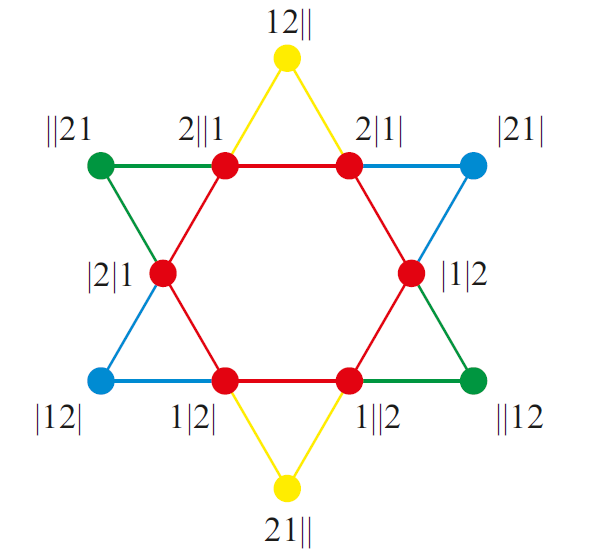
\includegraphics[width=170pt]{img/tolgraph-2balls.png}
    \caption{Vsi londonski grafi s $p=3$ in $n=2$ so ravninski.}
    \label{fig:graf-2krogli}
\end{figure}

Če si sedaj pogledamo problem londonskega stolpa s tremi kroglami ($n=3$), na podoben način kot za dve krogli dobimo sledečo shemo:

\begin{equation}
\label{eq:grafi-3krogle}
\begin{matrix}
    & & L & & & & \\
    & & \parallel & & & & \\
    L_{122}^3 & \subset & L_{123}^3 & \subset & L_{133}^3 & & \\
    \cap & & \cap & & \cap & & \\
    L_{222}^3 & \subset & L_{223}^3 & \subset & L_{233}^3 & \subset & L_{333}^3 \\
    & & & & & & \parallel \\
    & & & & & & O^3_3 \\
\end{matrix}
\end{equation}

\smallskip

Videli smo že, da je klasični londonski graf $L$ ravninski. Torej je ravninski tudi njegov podgraf $L_{122}^3$, saj do njega pridemo tako, da iz $L$ zbrišemo tistih šest vozlišč, kjer so vse tri krogle na največji palici, in pripadajoče povezave. 
Če pa grafu $L$ dodamo vozlišča, kjer so vse tri krogle na srednji palici, lahko s slike~\ref{} vidimo, da je tudi $L_{133}^3$ ravninski.

\begin{trditev}
    Naj bo $p=3$. Tedaj so ravninski londonski grafi natanko grafi $L_h^2, L_{122}^3, L_{123}^3$ in $L_{133}^3$.
\end{trditev}

\begin{opomba}
    Še vedno predpostavljamo, da so londonski grafi povezani, torej zadostujejo pogoju~\eqref{eq:pogoj-povezanosti}.
\end{opomba}

\begin{proof}
    Videli smo že, da so grafi $L_h^2, L_{122}^3, L_{123}^3$ in $L_{133}^3$ ravninski. Dokazati moramo, da vsi ostali grafi za $n=3$ in vsi grafi za $n \geq 4$ niso ravninski. Pri tem nam bo v pomoč izrek~\ref{izr:kuratowski}, ki pravi, da je graf ravninski natanko tedaj, ko ne vsebuje subdivizije $K_5$ ali $K_{3,3}$. A v grafu $L_{222}^3$ lahko najdemo subdivizijo $K_{3,3}$, ki je na sliki~\ref{fig:L222-subdivizija} prikazana z rdečo barvo. 
    \begin{figure}[h]
        \centering
        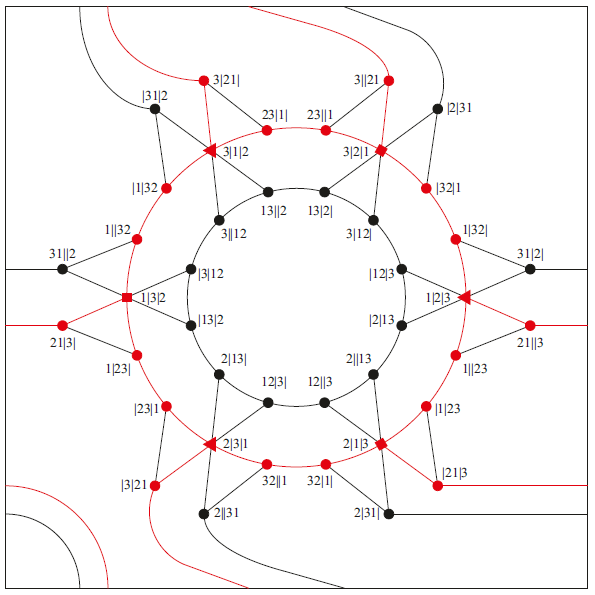
\includegraphics[width=400pt]{img/tolgraph-O^3_222-subdivision.png}
        \caption{Graf $L_{222}^3$ vsebuje subdivizijo $K_{3,3}$.}
        \label{fig:L222-subdivizija}
    \end{figure}
    Iz tega po izreku~\ref{izr:kuratowski} sledi, da $L_{222}^3$ ni ravninski. Ker vsi preostali grafi z $n = 3$ vsebujejo graf $L_{222}^3$ (kot lahko vidimo na shemi~\eqref{eq:grafi-3krogle}), tudi $L_{223}^3, L_{233}^3, L_{333}^3=O^3_3$ niso ravninski.
    
    Dokazati moramo le še, da tudi londonski grafi za $n\geq 4$ niso ravninski.
    Ker $L_{222}^3$ ni ravninski in je vsebovan v grafu $L_{222}^4$, sledi, da $L_{222}^4$ ni ravninski. Pokazali bi lahko, da tudi graf $L_{133}^4$ ni ravninski, vendar si pri tem ne moremo pomagati z njegovim ravninskim podgrafom $L_{133}^3$, zato bi morali znotraj $L_{133}^4$ poiskati subdivizijo $K_{3,3}$. Ta naloga je precej mučna zaradi velikosti grafa, zato jo bomo izpustili.
    Ker mora vsak graf $L_h^4$ vsebovati ali $L_{133}^4$ ali $L_{222}^4$, ki nista ravninska, to sledi tudi za preostale grafe z $n=4$.
    
    Za $n \geq 4$ torej noben graf ni ravninski, saj vsak $L_h^n$ dobimo z dodajanjem krogel enemu izmed $L_h^4$, za katere pa zdaj vemo, da niso ravninski.
\end{proof}

\begin{opomba}
    [TODO] toroidalnost
\end{opomba}

\subsection{Simetrije londonskega stolpa}

Zamislimo si za trenutek problem londonskega stolpa, pri katerem so vse palice različne višine. Simetrije pripadajočega grafa so ravno vse možne permutacije barv krogel.
Če pa pri našem problemu obstaja nekaj palic, ki so enake višine, pa so simetrije grafa tudi permutacije palic enake višine.
V temu poglavju bomo najprej omenili simetrije klasičnega problema londonskega stolpa, nato pa preučili še simetrije nekaterih ostalih problemov s tremi palicami, z uporabo simetrijskih lastnosti pa bomo potem sklepali nekaj več o lastnostih pripadajočih grafov.

Pri klasičnem problemu londonskega stolpa imamo $3$ palice različne višine, torej so edine možne simetrije permutacije barv krogel. Spomnimo se, naloga je sestavljena iz začetnega stanja krogel in končnega stanja krogel, matematično jo torej lahko opišemo kot urejen par dveh možnih stanj. Klasični problem ima 36 možnih stanj, torej imamo $36 \cdot 35$ možnih nalog. 

% slovar
\section*{Slovar strokovnih izrazov}

%\geslo{}{}
%
%\geslo{}{}
%

% seznam uporabljene literature
\begin{thebibliography}{99}

\bibitem{bib:tohmyths} A. M. Hinz, S. Klavžar, U. Milutinović in C. Petr, \emph{The Tower of Hanoi – Myths and Maths}, Birkhäuser, Basel, 2013.

\bibitem{bib:potocnik} P. Potočnik, \emph{Zapiski predavanj iz Diskretne Matematike I}, 1.~izdaja, [ogled 29.~12.~15], dostopno na \url{http://www.fmf.uni-lj.si/~potocnik/Ucbeniki/DM-Zapiski2010.pdf}

\bibitem{bib:wikishal} \emph{Tim Shallice}, v: Wikipedia: The Free Encyclopedia, [ogled 8.~10.~2015], dostopno na\\ \url{https://en.wikipedia.org/wiki/Tim_Shallice}.

\bibitem{bib:wikihamilpath} \emph{Hamiltonian path}, v: Wikipedia: The Free Encyclopedia, [ogled 28.~12.~2015], dostopno na \url{https://en.wikipedia.org/wiki/Hamiltonian_path}.
\end{thebibliography}

\end{document}

